\documentclass{article}
\usepackage{tikz}
\usetikzlibrary{shapes,positioning}
\begin{document}
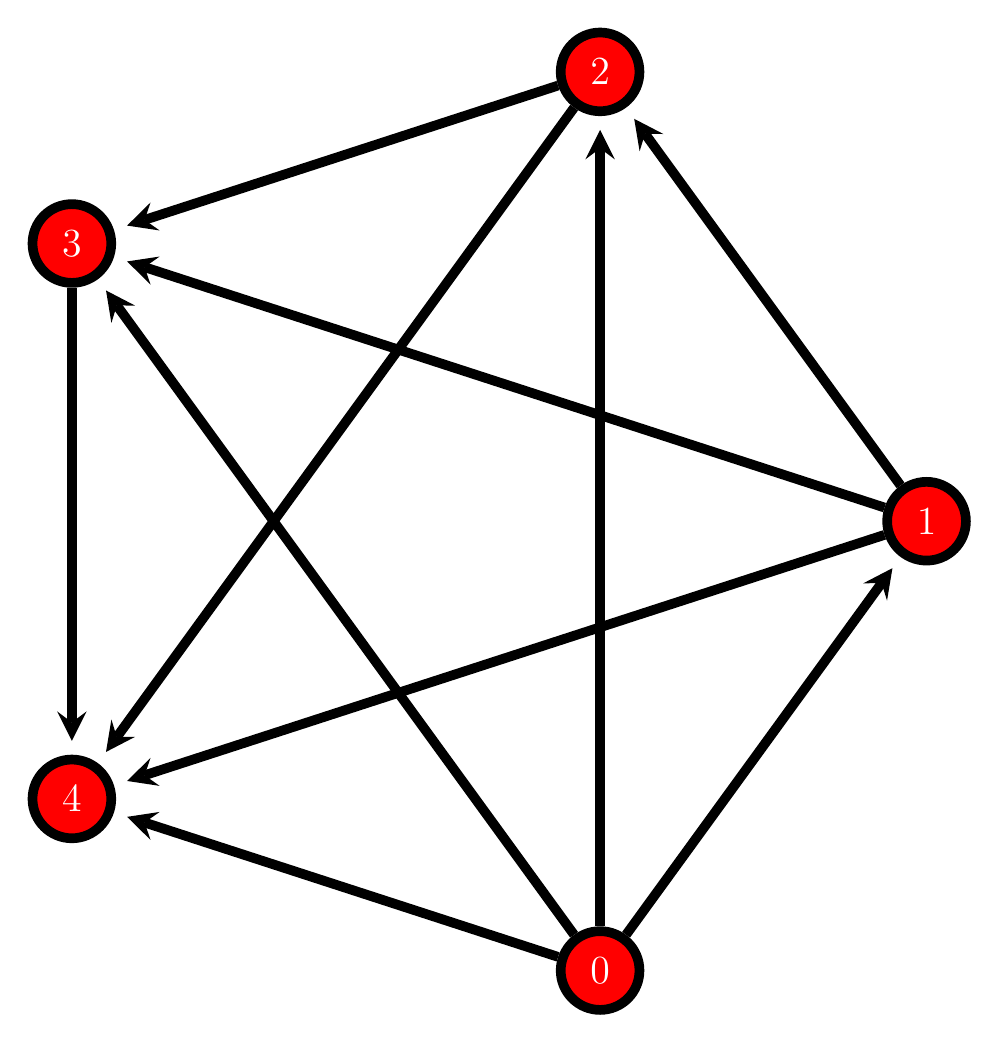
\begin{tikzpicture}[ every node/.style={circle,draw,minimum size=10mm, font=\Large, inner sep=1mm, text=white,  fill=red}, level/.style={sibling distance=50mm/#1}, level 2/.style={sibling distance=30mm}, level 3/.style={sibling distance=20mm}, thick,>=stealth, ->, line width=3.5pt,shorten >=5pt]
\node (v0) at (-72.0:6cm) {0};
\node (v1) at (0.0:6cm) {1};
\node (v2) at (72.0:6cm) {2};
\node (v3) at (144.0:6cm) {3};
\node (v4) at (216.0:6cm) {4};
\draw (v0) -> (v1);
\draw (v0) -> (v2);
\draw (v0) -> (v3);
\draw (v0) -> (v4);
\draw (v1) -> (v2);
\draw (v1) -> (v3);
\draw (v1) -> (v4);
\draw (v2) -> (v3);
\draw (v2) -> (v4);
\draw (v3) -> (v4);
\end{tikzpicture}
\end{document}